\chapter{Related work}
\label{chapter3}
\thispagestyle{plain}
There are a number of other similar digital platforms on the internet which provide booking services online. Among them Booking\footnote{www.Booking.com is a travel meta search engine for lodging reservations.} and AirBnB are the most well known. Observation of similar platforms help us in understanding the shortcomings and lacking features/functionalities which can potentially differentiate our platform from the existing platforms. In addition we can identify the most essential functionalities that our platform shall provide for the end users (a.k.a. "Must-have features"). 

Since development team did not have access to Software code and assets of the competitor platforms, the team analyzed their software from User Experience(UX) perspective. The team found out, practices used by the competitor platforms toward their customers are not always aligned with end users expectations from these platforms, this concept is  defined as \textit{Dark patterns} among UX design researchers community.

According to \citeauthor{dark_pattern} the term \textit{Dark patterns} refers to instances where designers use their knowledge of human behavior (e.g., psychology)and the desires of end users to implement deceptive functionality that is not in the user’s best interest\cite{dark_pattern}. In addition \citeauthor{dark_pattern} classify \textit{Dark patterns} as follows:

\begin{itemize}
  \item Bait and Switch disguised Ad: User sets out to do one thing, but a different, undesirable thing happens instead. Adverts that are disguised as other kinds of content or navigation, in order to get User to click on them.
  \item Forced Continuity: When Users free trial with a service comes to an end and Users credit card silently starts getting charged without any warning. In some cases this is made even worse by making it difficult to cancel the membership.
  \item Friend Spam: The product asks for Users email or social media permissions under the pretence it will be used for a desirable outcome (e.g. finding friends), but then spams all Users contacts in a message that claims to be from the user.
  \item Hidden Costs: User get to the last step of the checkout process, only to discover some unexpected charges have appeared, e.g. delivery charges, tax, etc.
  \item misdirection: The design purposefully focuses users attention on one thing in order to distract him/her attention from another.
  \item Price comparison prevention: The retailer makes it hard for user to compare the price of an item with another item, so user cannot make an informed decision.
  \item privacy zuckering: Users are tricked into publicly sharing more information about themselves than they really intended to. Named after Facebook CEO Mark Zuckerberg.
  \item roach model: The design makes it very easy for user to get into a certain situation, but then makes it hard for user to get out of it (e.g. a subscription).
  \item Sneak into basket: User attempts to purchase something, but somewhere in the purchasing journey the site sneaks an additional item into the users basket, often through the use of an opt-out radio button or checkbox on a prior page
  \item Trick questions: User responds to a question, which, when glanced upon quickly appears to ask one thing, but if read carefully, asks another thing entirely.
\end{itemize}


The development team analyzed competitor platforms, by conducting an online survey from a community of one hundred digital platform users among company employees. The result showed 85\% already experienced either one or multiple forms of \textit{Dark patterns} practices and they were dissatisfied with their experience. The dominant categories of malpractices from survey are as follows:
\begin{itemize}
  \item Misleading price sorting
  \item Incoherent rating system, some platforms categorize multiple aspects of hospitality experience, however they only show the best average rating
  \item Misleading reviews on front/first page, some platforms tend to sort reviews in a way which prioritize positive reviews on the first page
\end{itemize}


Here there are some examples of usage of \textit{Dark patterns}. 
Figure \ref{fig:dark_pattern_1} and \ref{fig:dark_pattern_2} illustrate a case of \textit{Misdirection} by a digital platform, in this case viewers are mislead into believing that the offer the platform purposes is time limited (sense of emergency) and the viewer may lose the chance in case of hesitation, which is not the case. 

%For instance some booking platforms mislead their viewers into believing that the offer they purpose is time limited (sense of emergency) and the viewer may lose the chance in case of hesitation (figure \ref{fig:dark_pattern_1}), this anti design pattern falls under category of \textit{Misdirection} by the platform. 

\begin{figure} 
\centering
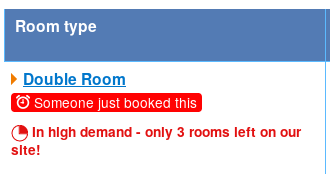
\includegraphics[width=8cm]{pictures/dark_pattern1.png}
\caption{Example of a Dark pattern in UX design}
Figure illustrating one type of Dark Patterns used by a booking platform
\label{fig:dark_pattern_1}
\end{figure}

\begin{figure} 
\centering
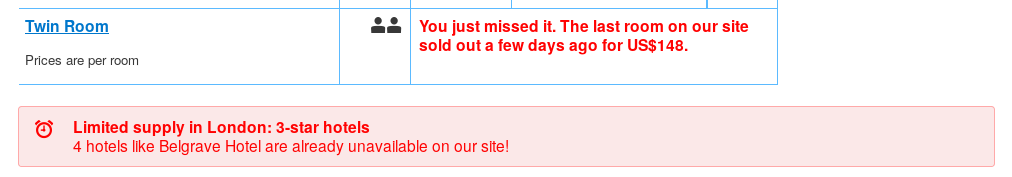
\includegraphics[width=14cm]{pictures/dark_pattern2.png}
\caption{Example of a Dark pattern in UX design}
Figure illustrating one type of Dark Patterns used by a booking platform
\label{fig:dark_pattern_2}
\end{figure}

Final conclusion drafted from the survey indicates, while in the short run usage of \textit{Dark patterns} practices might improve short term profitability of the platform through increased number of bookings, in the long run it will damage reputation of company as well as customer loyalty to the platform, which lead customers into migrating to another platform. The development team concluded that the differentiating factor for our platform is "customer first" approach. By adopting "customer first" approach the \textit{Dark patterns} practices are avoided altogether, while the emphasis is to build a trust and log lasting relationship between platform end users and the platform owners.




\citeauthor{web_security} study \cite{web_security} examines various modes of attacks on websites including cross site scripting(XSS), Sql Injection as well as mitigation techniques against such attacks which author classifies as extensive testing of security and software verification techniques. The important viewpoint which needs to be addressed is the \textit{insecure information flow} of web application which can introduce vulnerabilities.  
For this purpose we used mitigation techniques against SQL injection attacks by using \textit{Spring} framework's prepared statement. Furthermore the design of the back-end system follows guidelines which incorporate cleansed(validated) data which is only accessible through tested APIs which are controlled by \textit{spring} authentication mechanisms in order to deny access to unauthorized usage of back-end data.  
Figure \ref{fig:spring_sec_1} illustrates one of the mitigation techniques against Unauthorized requests.
The steps which are implemented by Spring Security is as follows:

\begin{enumerate}
  \item the FilterSecurityInterceptor obtains an Authentication from the SecurityContextHolder.
  \item FilterSecurityInterceptor creates a FilterInvocation from the HttpServletRequest, HttpServletResponse, and FilterChain that are passed into the FilterSecurityInterceptor.
  \item lNext, it passes the FilterInvocation to SecurityMetadataSource to get the ConfigAttributes.
  \item Finally, it passes the Authentication, FilterInvocation, and ConfigAttributes to the AccessDecisionManager.
  \item If authorization is denied, an AccessDeniedException is thrown. In this case the ExceptionTranslationFilter handles the AccessDeniedException.
  \item If access is granted, FilterSecurityInterceptor continues with the FilterChain which allows the application to process normally.
\end{enumerate}
  

\begin{figure} 
\centering
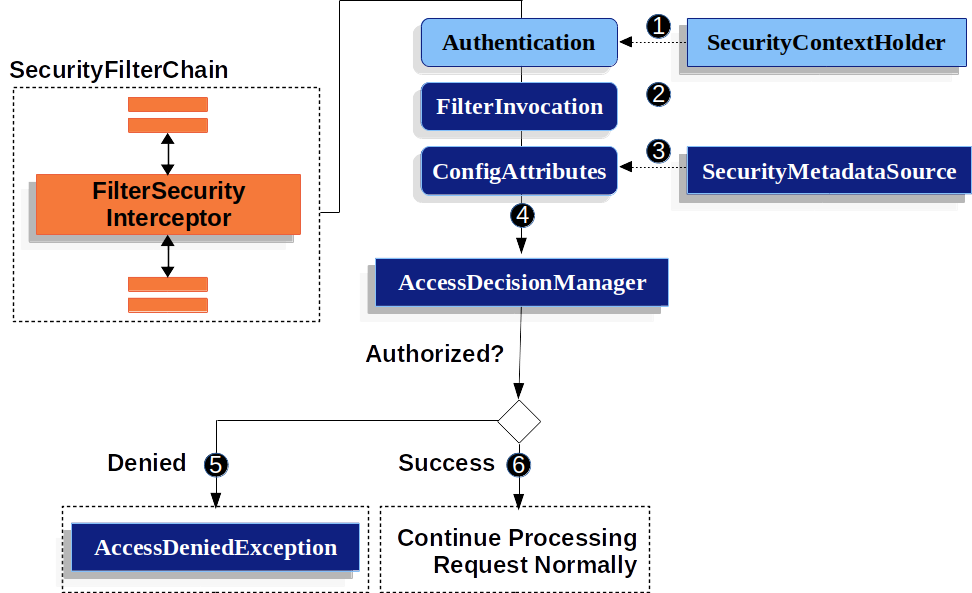
\includegraphics[width=14cm]{pictures/spring_sec_1.png}
\caption{Spring Authorization of HttpServletRequest}
Figure handling of Unauthorized HttpServletRequest.
\label{fig:spring_sec_1}
\end{figure}






%force their viewers to believe there is a sense of emergency and the available properties may be booked by another customer at any second. 

%In addition the usage of so called <Dark patterns> by the platforms which offer booking, is a practice that is avoided entirely in the User experience design of our website.
%\section{Related work}
%\subsection{blah blah}\label{sec:blah_blah}

